\section{Topología en el espacio euclídeo}
\begin{definición}[Longitud o Norma euclídea]
    Se denomina \textbf{longitud} o \textbf{norma euclídea} de un vector $\vec{x} = (x_1, x_2, \ldots, x_n) \in \mathbb{R}^n$ al númeor real mayor o igual que cero definido por $$\|\vec{x}\| = \sqrt{x_1^2 + x_2^2 + \ldots + x_n^2}.$$
\end{definición}

\begin{definición}[Distancia euclídea]
    Se llama \textbf{distancia euclídea} entre dos vectores $\vec{x} = (x_1, x_2, \ldots, x_n)$ y $\vec{y} = (y_1, y_2, \ldots, y_n)$ al número real mayor o igual que 0 definido por:
    \[
        d(\vec{x}, \vec{y}) = \|\vec{x} - \vec{y}\| = \left( \sum_{i = 1}^{n} (x_i - y_i)^2 \right)^{\frac{1}{2}}
    \]
\end{definición}

\begin{definición}[Producto escalar euclídeo]
    Se llama \textbf{producto escalar euclídeo} entre dos vectores $\vec{x} = (x_1, x_2, \ldots, x_n)$ y $\vec{y} = (y_1, y_2, \ldots, y_n)$ al número real, no necesariamente positivo, definido por:
    $$\langle \vec{x}, \vec{y} \rangle = x_1 y_1 + x_2 y_2 + \ldots + x_n y_n = \sum_{i = 1}^{n} x_i y_i.$$
\end{definición}


\begin{teorema}
    \begin{enumerate}
        \item $\langle \vec{x}, \vec{y} \rangle \geq 0 \quad \forall \vec{x}, \vec{y} \in \mathbb{R}^n$.
        \item $\langle \vec{x}, \vec{y} \rangle = 0 \Leftrightarrow \vec{x} = \vec{0}$ o $\vec{y} = \vec{0}$.
        \item $\forall \vec{x}, \vec{y}, \vec{z} \in \mathbb{R}^n \text{ se cumple que } \langle \vec{x} + \vec{y}, \vec{z} \rangle = \langle \vec{x}, \vec{z} \rangle + \langle \vec{y}, \vec{z} \rangle$.
        \item $\langle \alpha \vec{x}, \vec{y} \rangle = \alpha \langle \vec{x}, \vec{y} \rangle$ para todo $\alpha \in \mathbb{R}$.
        \item $\langle \vec{x}, \vec{y} \rangle = \langle \vec{y}, \vec{x} \rangle$.
    \end{enumerate}
\end{teorema}

\begin{teorema}
    Para cualesquiera $x, \in \mathbb{R}^2$ se verifica que $\langle x, y\rangle = \|\vec{x}\| \|\vec{y}\| \cos(\theta)$, donde $\theta$ es el ángulo entre los vectores $\vec{x}$ y $\vec{y}$.
\end{teorema}
\begin{proof}
    Dados dos vectores \( x \) e \( y \) de \( \mathbb{R}^2 \), que supondremos distintos de 0 (pues si uno de ellos es 0 el resultado es inmediato), consideremos el triángulo de vértices \( 0 \), \( x \), \( y \):
    
    
    \begin{center}
    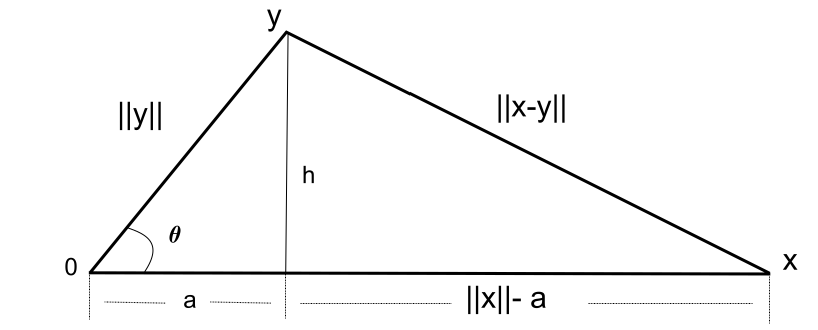
\includegraphics[width=0.5\textwidth]{Graphics/triangulo.png} % Reemplaza con tu gráfico si quieres incluir uno.
    \end{center}
    Utilizando trigonometría elemental, tenemos que:
    \[
    \cos \theta = \frac{a}{\|y\|}
    \]

    Además, usando el teorema de Pitágoras, tenemos que:
    $$ \|y\|^2 = a^2 + h^2 \implies \|y\|^2 - a^2 = h^2 = \|x - y\|^2 - (\|x\| - a)^2$$

    Con lo que:
    \[
    \|x - y\|^2 = \|y\|^2 - a^2 + \|x\|^2 - 2a\|x\| + a^2 = \|y\|^2 + \|x\|^2 - 2a\|x\|
    \]

    Usando que \( a = \|y\|\cos\theta \), obtenemos:
    \[
    \|x - y\|^2 = \|x\|^2 + \|y\|^2 - 2\|x\|\|y\|\cos\theta
    \]

    Si ahora usamos las propiedades del producto interior, obtenemos que:
    \[
    \|x - y\|^2 = \langle x - y, x - y \rangle = \|x\|^2 - 2\langle x, y \rangle + \|y\|^2
    \]

    De donde se deduce, teniendo en cuenta el valor previamente obtenido de \( \|x - y\|^2 \), que:
    \[
    \langle x, y \rangle = \|x\| \|y\| \cos\theta
    \]
\end{proof}

\begin{definición}[Vectores ortogonales]
    Se dice que dos vectores \( \vec{x} \) y \( \vec{y} \) son \textbf{ortogonales} si $\langle \vec{x}, \vec{y} \rangle = 0$.
\end{definición}

\begin{proposición}[Propiedades de la norma euclídea]
    \begin{enumerate}
        \item $\|\vec{x}\| \geq 0 \quad \forall \vec{x} \in \mathbb{R}^n$.
        \item $\|\vec{x}\| = 0 \Leftrightarrow \vec{x} = \vec{0}$.
        \item $\|\alpha \vec{x}\| = |\alpha| \|\vec{x}\|$ para todo $\alpha \in \mathbb{R}$.
        \item $\|\vec{x} + \vec{y}\| \leq \|\vec{x}\| + \|\vec{y}\| \quad \forall \vec{x}, \vec{y} \in \mathbb{R}^n$ (desigualdad triangular).
    \end{enumerate}
\end{proposición}

\begin{teorema}[Desigualdad de Cauchy-Schwarz]
    Sea \( \vec{x}, \vec{y} \in \mathbb{R}^n \). Entonces se cumple que:
    \[
        |\langle \vec{x}, \vec{y} \rangle| \leq \|\vec{x}\| \|\vec{y}\|
    \]

    Equivalentemente 
    $$\left\|\sum_{i=1}^{n} x_i y_i\right\| \leq \sqrt{\sum_{i=1}^{n} x_i^2} \sqrt{\sum_{i=1}^{n} y_i^2}$$
    
\end{teorema}

\begin{proof}
    Fijemos $\vec{x}$ y $\vec{y} \in \mathbb{R}^n$. Para cada $\alpha \in \mathbb{R}$ se tiene que 
    $$\langle \alpha \vec{x} + \vec{y}, \alpha \vec{x} + \vec{y} \rangle  = \alpha^2 \langle , \rangle + 2\alpha \langle x, y\rangle + \langle y, y \rangle \geq 0$$
    Si tomamos $A = \langle \vec{x}, \vec{x} \rangle$, $B = 2\langle \vec{x}, \vec{y} \rangle$ y $C = \langle \vec{y}, \vec{y} \rangle$, tenemos que: 
    $$A\alpha^2 + B\alpha + C \geq 0 \quad \forall \alpha \in \mathbb{R}$$
    Entoncespodemos distinguir dos casos:
    \begin{enumerate}
        \item Si \( A = 0 \), entonces \( \vec{x} = \vec{0} \) y la desigualdad es trivial.
        \item Si \( A > 0 \), entonces la desigualdad anterior es una ecuación cuadrática en \( \alpha \), y por las propiedades del producto escalar es necasrio que su discriminantes sea no positivo, pues de lo contrario tendría dos raíces reales distintias y entonces la ecuacion tomaría algún valor negativo 
        $$\implies D = B^2 - 4AC \leq 0 \iff B^2 \leq 4AC \iff 4\langle \vec{x}, \vec{y} \rangle^2 \leq 4\langle \vec{x}, \vec{x} \rangle \langle \vec{y}, \vec{y} \rangle = 4\|x\|^2 \|y\|^2$$
    \end{enumerate}

\end{proof}

\begin{proposición}[Propiedades de la distancia euclídea]
    \begin{enumerate}
        \item $d(\vec{x}, \vec{y}) \geq 0 \quad \forall \vec{x}, \vec{y} \in \mathbb{R}^n$.
        \item $d(\vec{x}, \vec{y}) = 0 \Leftrightarrow \vec{x} = \vec{y}$.
        \item $d(\vec{x}, \vec{y}) = d(\vec{y}, \vec{x})$.
        \item $d(\vec{x}, \vec{z}) \leq d(\vec{x}, \vec{y}) + d(\vec{y}, \vec{z})$ (desigualdad triangular).
    \end{enumerate}
\end{proposición}

\begin{definición}[Métrica]
    Se llama \textbf{métrica} sobre un conjunto arbitrario $M$ a cualquier aplicación $d: M \times M \to \mathbb{R}$ que cumple las siguientes propiedades:
    \begin{enumerate}
        \item $d(x, y) \geq 0 \quad \forall x, y \in M$.
        \item $d(x, y) = 0 \Leftrightarrow x = y$.
        \item $d(x, y) = d(y, x)$.
        \item $d(x, z) \leq d(x, y) + d(y, z)$ (desigualdad triangular).
    \end{enumerate}
\end{definición}

\begin{definición}[Espacio métrico]
    Se llama \textbf{espacio métrico} a un par $(M, d)$ donde $M$ es un conjunto no vacío y $d$ es una métrica sobre $M$.
\end{definición}

\ejemplo{
    Vemos algunos ejemploes de métricas: 
    \begin{enumerate}
        \item La métrica euclídea en $\mathbb{R}^n$ 
        \item $d_1(x, y) = \sum_{i = 1}^{n} |x_i - y_i|$ 
        \item $d_\infty(x, y) = \max_{i = 1, \ldots, n} |x_i - y_i|$
        \item $d(f, g) = \int_{a}^{b} |f(x) - g(x)| dx$ para funciones $f, g: [a, b] \to \mathbb{R}$.
        \item $d_{\infty}(f, g) = \max_{x \in [a, b]} |f(x) - g(x)|$ para funciones $f, g: [a, b] \to \mathbb{R}$.
        \item $d(x, y) = \begin{cases}
            0 & \text{si } x = y \\
            1 & \text{si } x \neq y
        \end{cases}$, que se conoce como la \textbf{métrica discreta}.
    \end{enumerate}
}

\begin{definición}[Diámetro]
    Se llama \textbf{diámetro} de un subconjunto $S$ de un espacio métrico $(M, d)$ a
    $$diam(S) = \sup\{d(x, y) \mid x, y \in S\}$$
    si el conjunto de números reales $\{d(x,y) : x,y \in S\}$ es acotado superiormente y se define $diam(S) = +\infty$ en caso contrario.Cual del diámetro es ifnito se dice que el conjunto es \textbf(acotado);
\end{definición}

\begin{definición}[Norma]
    Sea $V$ un espacio vectorial sobre $\mathbb{R}$. Se llama \textbf{norma} en $V$ a toda aplicación $\|\cdot\|: V \to \mathbb{R}$ que cumple las siguientes propiedades:
    \begin{enumerate}
        \item $\|\vec{x}\| \geq 0 \quad \forall \vec{x} \in V$.
        \item $\|\vec{x}\| = 0 \Leftrightarrow \vec{x} = \vec{0}$.
        \item $\|\alpha \vec{x}\| = |\alpha| \|\vec{x}\|$ para todo $\alpha \in \mathbb{R}$.
        \item $\|\vec{x} + \vec{y}\| \leq \|\vec{x}\| + \|\vec{y}\|$ (desigualdad triangular).
    \end{enumerate}
\end{definición}

\ejemplo{
    \begin{enumerate}
        \item $\|\vec{x}\| = |x|$
        \item $\|\vec{x}\|_2 = \left(\sum_{j = 1}^{n} x_j^2\right)^{\frac{1}{2}}$ (norma euclídea).
        \item $\|\vec{x}\|_1 = \sum_{j = 1}^{n} |x_j|$ (norma $l^1$).
        \item $\|\vec{x}\|_\infty = \max_{j = 1, \ldots, n} |x_j|$ (norma $l^\infty$).
        \item $\|f\|_{\infty} = \max_{x \in [a, b]} |f(x)|$ para funciones $f: [a, b] \to \mathbb{R}$.
    \end{enumerate}
}

\begin{definición}[Producto escalar o interior]
    Llamaremos producto escalar o producto interior en $V$ a toda aplicación $\langle \cdot, \cdot \rangle: V \times V \to \mathbb{R}$ que cumple las siguientes propiedades:
    \begin{enumerate}
        \item $\langle \vec{x}, \vec{y} \rangle \geq 0 \quad \forall \vec{x}, \vec{y} \in V$.
        \item $\langle \vec{x}, \vec{x} \rangle = 0 \Leftrightarrow \vec{x} = \vec{0}$.
        \item $\langle \vec{x}, \vec{y} \rangle = \langle \vec{y}, \vec{x} \rangle$.
        \item $\langle \alpha \vec{x}, \vec{y} \rangle = \alpha \langle \vec{x}, \vec{y} \rangle$ para todo $\alpha \in \mathbb{R}$.
        \item $\langle \vec{x} + \vec{y}, \vec{z} \rangle = \langle \vec{x}, \vec{z} \rangle + \langle \vec{y}, \vec{z} \rangle$ para todo $\vec{x}, \vec{y}, \vec{z} \in V$.
    \end{enumerate}
\end{definición}

\begin{definición}[Igualdad del paralelogramo]
    Sea una norma $\|\cdot\|$ en un espacio vectorial $V$. Se dice que la norma cumple la \textbf{igualdad del paralelogramo} si la norma procede de un producto escalar
    $$\|\vec{x} + \vec{y}\|^2 + \|\vec{x} - \vec{y}\|^2 = 2\|\vec{x}\|^2 + 2\|\vec{y}\|^2$$
\end{definición}
\begin{proof}
    $$\|\vec{x} + \vec{y}\|^2 + \|\vec{x} - \vec{y}\|^2 = \langle \vec{x} + \vec{y}, \vec{x} + \vec{y} \rangle + \langle \vec{x} - \vec{y}, \vec{x} - \vec{y} \rangle = $$
    $$ = \|\vec{x}\|^2 + \langle \vec{x}, \vec{y} \rangle + \langle \vec{y}, \vec{x} \rangle + \|\vec{y}\|^2 + \|\vec{x}\|^2 - \langle \vec{x}, \vec{y} \rangle - \langle \vec{y}, \vec{x} \rangle + \|\vec{y}\|^2 = 2\|\vec{x}\|^2 + 2\|\vec{y}\|^2$$
\end{proof}

\begin{definición}[Bola abierta]
    Dados $x_0 \in \mathbb{R}^n$ y un número real $r > 0$, llamamos \textbf{bola abierta} de centro $x_0$ y radio $r$ al conjunto
    $$B(x_0, r) = \{x \in \mathbb{R}^n \mid d(x, x_0) < r\}$$
    donde $d$ es la métrica que se está considerando en $\mathbb{R}^n$.
\end{definición}

\begin{definición}[Conjunto abierto]
    Se dice que un conjunto $A \subset \mathbb{R}^n$ es \textbf{abierto} si para todo punto $x_0 \in A$ existe un número real $r > 0$ tal que $B(x_0, r) \subset A$.
\end{definición}

\begin{proposición}[Propiedades de los conjuntos abiertos]
    \begin{enumerate}
        \item El conjunto vacío y el espacio euclídeo $\mathbb{R}^n$ son abiertos.
        \item La unión de abiertos es un abierto
        \item La interseccion finita de abiertos es un abierto.
    \end{enumerate}
\end{proposición}

\begin{definición}[Punto abierto]
    Se dice que un punto $x \in S \subset \mathbb{R}^n$ es un \textbf{punto abierto} de $S$ si existe una bola abierta $B(x, r)$ tal que $B(x, r) \subset S$. Denotamos por $S^\circ$ al conjunto de los puntos abiertos de $S$.
\end{definición}

\begin{observación}
    $S^\circ$ puede ser vacío, por ejemplo si $S$ es un subconjunto con un solo punto
\end{observación}

\begin{proposición}[Propiedades de los puntos abiertos]
    \begin{enumerate}
        \item $S^\circ$ es el mayor abierto contenido en $S$
        \item $S^\circ$ es la unión de todos los abiertos contenidos en $S$.
        \item $S$ es abierto si y solo si $S = S^\circ$.
    \end{enumerate}
\end{proposición}
\begin{proof}
    \begin{enumerate}
        \item $S^\circ$ es abierto, pues dado $x \in S^\circ$, existe $r > 0$ tal que $B(x, r) \subset S$. Entonces sucede que $B(x, r) \subset S^\circ$, pues al ser $B(x, r)$ un abierto, entonces $B(x, r) = [B(x, r)]^{\circ} \subset S^\circ$. Por otra parte, si $A$ es un abierto de $\mathbb{R}^n$ contenido en $S$, entonces para todo punto de A hay una bola centrada en él contenida en $A$ y por lo tanto en $S$, lueg todos los puntos de $A$ están en $S^\circ$
        \item Es claro que el mayor abierto contenido en $S$ es la unión de todos los abiertos contenidos en $S$
        \item Si $S$ es abierto, entonces él es el mayor abierto contenido en $S$, luego $S = S^\circ$. Por otra parte, si $S = S^\circ$, entonces $S$ es abierto, pues para todo punto $x \in S$, existe una bola abierta $B(x, r)$ tal que $B(x, r) \subset S$, luego $S$ es abierto.	
    \end{enumerate}
\end{proof}

\begin{definición}[Bola cerrada]
    Dados $x_0 \in \mathbb{R}^n$ y un número real $r > 0$, llamamos \textbf{bola cerrada} de centro $x_0$ y radio $r$ al conjunto
    $$\overline{B}(x_0, r) = \{x \in \mathbb{R}^n \mid d(x, x_0) \leq r\}$$
\end{definición}
\begin{proof}
    
\end{proof}
